\documentclass{article}
\usepackage[utf8]{inputenc}

\title{Method \& Result}
\author{Zeyu Xu}
\date{May 2019}

\usepackage{natbib}
\usepackage{graphicx}
\usepackage{color}
\usepackage{booktabs}
\usepackage{cases}
\usepackage{amsmath}

\begin{document}

\maketitle
\begin{abstract}
Based on Schelling's Segregation model, people's preference for neighbors of the same race will lead to segregation. But do people really consider population composition while making decisions on moving? What's the impact of homophily preference on people's moving decision within the city? This paper addresses those problems using a discrete choice model. The model makes prediction on the probability of moving between blocks based on the income level and population composition of blocks. Using the data of 62 blocks in Chicago from 2011 to 2017, the paper finds people are more willing to live with those of the same race. Besides, the paper also finds interesting difference between whites and blacks. While whites are not sensitive to the income level of blocks, blacks care about both the general income level and the income structure of blocks.
\par
\textbf{Keywords:} Segregation, Homophily Preference, Race, Chicago    
\end{abstract}
\newpage
\section{Method \& Data}
\subsection{Theoretical Model}
\par \ \ \ \ Based on the assumption that people care about the percentage of their ethnic group in the neighborhood they choose, I build a discrete choice model to describe the probability of an agent to move from one block to another:
\begin{eqnarray}
\triangle_{i,j,t} &=& \beta_1 \times (log(income_{j,t})-log(income_{i,t})) \nonumber\\
&\;&+\ \beta_2 \times (homophily_{j,t}-homophily_{i,t})\\ 
p_{i,j,t} &=& \frac{1}{1+e^{-\triangle_{i,j,t}}}\\
\hat{p}_{i,j,t} &=& (1-r)\times\frac{p_{i,j,t}}{\sum_{ke i} p_{i,k,t}}\\
P_t &=& 
\left[
\begin{array}{ccccc}
r & \hat{p}_{1,2,t} & \hat{p}_{1,3,t} & \cdots & \hat{p}_{1,n,t} \\
\hat{p}_{2,1,t} & r & \hat{p}_{2,3,t} & \cdots & \hat{p}_{2,n,t} \\
\vdots & \vdots & \vdots &  & \vdots \\
\hat{p}_{n-1,1,t} & \hat{p}_{n-1,2,t} & \hat{p}_{n-1,3,t} & \cdots & \hat{p}_{n-1,n,t}\\
\hat{p}_{n,1,t} & \hat{p}_{n,2,t} & \hat{p}_{n,3,t} & \cdots & r 
\end{array}
\right]
\end{eqnarray}
\par In this model, $P$ is the transition matrix of the population in blocks. $p_{i,j,t}$ is the rough probability that the agent moves from block $i$ to block $j$ at period $t$. Since we only care about the relative size of probability to move to different blocks, so we can scaled all $p$ to $(1-r)$ to ensure every row of $P$, which means the fraction of people moving to other block from one block, sums to 1. The parameter $r$ represents the ratio of people staying in the same block, which may result from unable to find satisfying house, unable to afford moving or other reasons. 
With the transition matrix, it’s easy to make prediction as follows:
\begin{eqnarray} 
\widehat{population}_{i,t+1} &=& population_{i,t} + \sum_{je i} population_{j,t}\times \hat{p}_{j,i,t} \nonumber\\ 
&\;& - \sum_{je i} population_{i,t}\times \hat{p}_{i,j,t} onumber\\ 
&=& \sum_{j} population_{j,t}\times \hat{p}_{j,i,t} 
\end{eqnarray}
\par The interpretation of the equation is straightforward. The $k$th row of the transition matrix depicts the flow out of population in block $k$ while the $k$th column of the transition matrix depicts the flow in of population from all blocks to block $k$. So one method to calculate the population in block $k$ is to take the difference between inflow and outflow population and add the population at the beginning. Another understanding of the matrix is the $k$th column of the matrix depicts the source of the population in block $k$ in next period, thus just multiply each probability by population of each block at the beginning.
\par The target of my model is to predict the migration within the city as accurately as possible. Since I don’t have the data of migration, the loss function should be based on the transition of population in each block to judge the quality of my model. If the population in the block is large enough, the transition matrix can make accurate prediction. If the population in the block is small, the actual moving population may differ to the prediction greatly since random factors affecting people’s migration have significant impact on blocks of small population. To avoid the noise of those blocks of small population, I use the weighted prediction error rate rather than average prediction error rate as the judgment criterion. Formally, the loss function is as follows:
\begin{eqnarray} 
Loss_{t+1} &=& \frac{1}{n} \sum_{i} \frac{|population_{i,t+1} - \widehat{population}_{i,t+1}|}{population_{i,t+1}} \times \frac{population_{i,t+1}}{\sum_j population_{j,t+1}} \nonumber \\
&=& \frac{1}{n} \sum_{i} \frac{|population_{i,t+1} - \widehat{population}_{i,t+1}|}{\sum_j population_{j,t+1}}
\end{eqnarray}
\par By minimizing loss function, I can get best parameters of my model with programming. Another advantage of that loss function is that we avoid infinite error rate caused by a block with 0 people of specific ethnic group because now I take the sum of population of the whole city at period $t$ as the denominator.

\subsection{Data Analysis}
\par \ \ \ \ This paper use American Community Survey Database to train the model. This database includes income and population composition statistics at different level. The database is public and can be accessed through the website of US Census Bureau.
\par This paper aims to study people’s migration within city, so I take Chicago as the target city and collect and analyze data at block level from 2011 to 2017. Blocks are represented by their zip codes. Since blacks and whites account for about 80 percent of total population in all blocks, I focus on those 2 ethnic groups and apply different parameters on different groups to see if they have significant difference that may lead to interesting inference.
\par For the summary of all variables grouped by years, please see the appendix. Table 1 summarizes population data grouped by year and Table 2 summarizes income data grouped by year. There is a significant character of population data, which is discussed below.
\par Graph 1 depicts the average black and white population in each block of 7 years. The heterogeneity of blocks is noteworthy here. Some blocks have less than 100 or even 0 blacks while some have more than 5 blacks. As for percentage, blacks account for less than 5\% in more than 1/4 of all blocks while account for over 90\% in some blocks. The statistics of whites suggests similar heterogeneity. Based on the theory, we should put more attention on those blocks with large enough population of specific ethnic groups since those with small population are much more noisy. The great heterogeneity supports the use of weighted average error rate.

\clearpage
\centerline{{\color{white} 100} Graph 1. Average black and white population in each block}
\begin{figure}[!h] 
\centering 
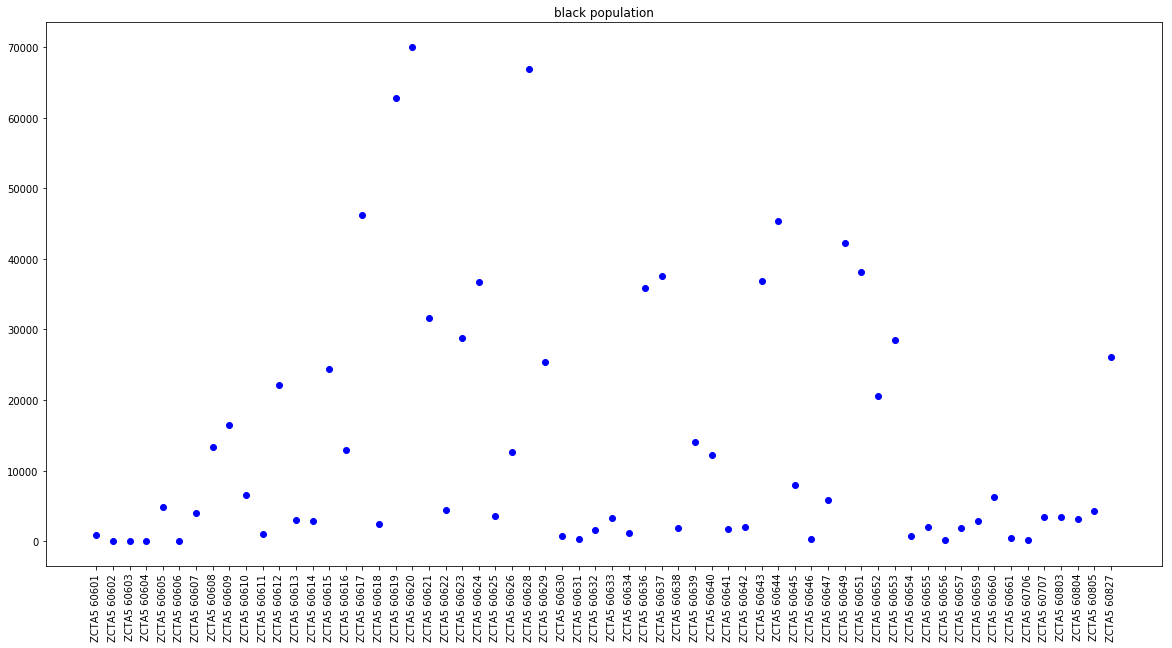
\includegraphics[width=1.2\textwidth]{graph1.png} 
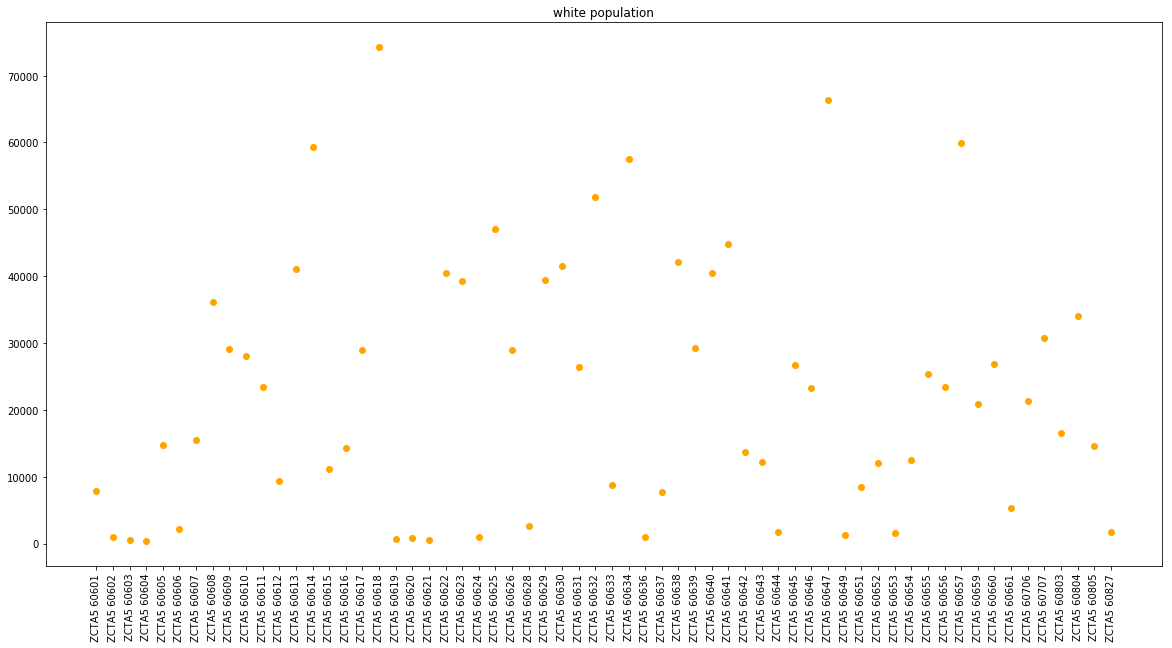
\includegraphics[width=1.2\textwidth]{graph2.png} 
\end{figure}

\section{Model Application \& Result}
\subsection{Result of Basic Model}
\ \ \ \ This part analyzes the prediction based on the basic model. Chicago has 62 blocks with nonzero population. In this part, I use mean income and exact percentage of specific ethnic group as features of the block. Given parameter, I can make prediction on population of each block based on their features last year and calculate the loss function. Researches have shown that blacks and whites have different tolerance to ethnic groups other than themselves (Charles, 2003\cite{Charles}; Zhang, 2011\cite{Zhang2011}), so it's better to set different parameters for them. Since there are other minorities and the model doesn't include transition matrix for income, it's better to make one-period prediction every year rather than simulate a series of data. After training, I get parameters as follows:
\begin{eqnarray}
r_{black} = 0.98, \beta_{1,black} = -5.05, \beta_{2,black} = 88.21 \nonumber \\
r_{white} = 0.98, \beta_{1,white} = -7.51, \beta_{2,white} = 14.95 \nonumber
\end{eqnarray}
\par The average prediction error rate for each block is depicted in Graph 2. I divided those blocks into 3 groups, small blocks, medium blocks and large blocks. Since the population of blacks and whites are different, I set different threshold for those groups. For both ethnic groups, the threshold of medium group is 2,500, but the threshold of large group is 15,000 for blacks and 25,000 for whites. As is shown in the graph. The prediction is accurate in medium and large blocks but is really unstable for small blocks, the reason is the relatively huge impact of random factors on small blocks. 
\par Table 3 summarizes weighted average error rate and average error rate for each of the 3 block groups from 2012 to 2017. The weighted average error rate is about 3\% for both ethnic group every year, suggesting the prediction is accurate.
\par The coefficient of income, i.e., $\beta_1$ is noteworthy. It's negative, suggesting that the higher the mean income of the block, the less likely that people move there. It is inconsistent with the intuition that people want to live where the income is higher. However, a possible reason for the negative coefficient is that a block with higher mean income may have higher housing price, which reduces the attraction of the block. We will discuss the role of income in the model in detail in next part.
\clearpage
\centerline{{\color{white} 100} Graph 2. Average prediction error rate for each block}
\begin{figure}[!h] 
\centering 
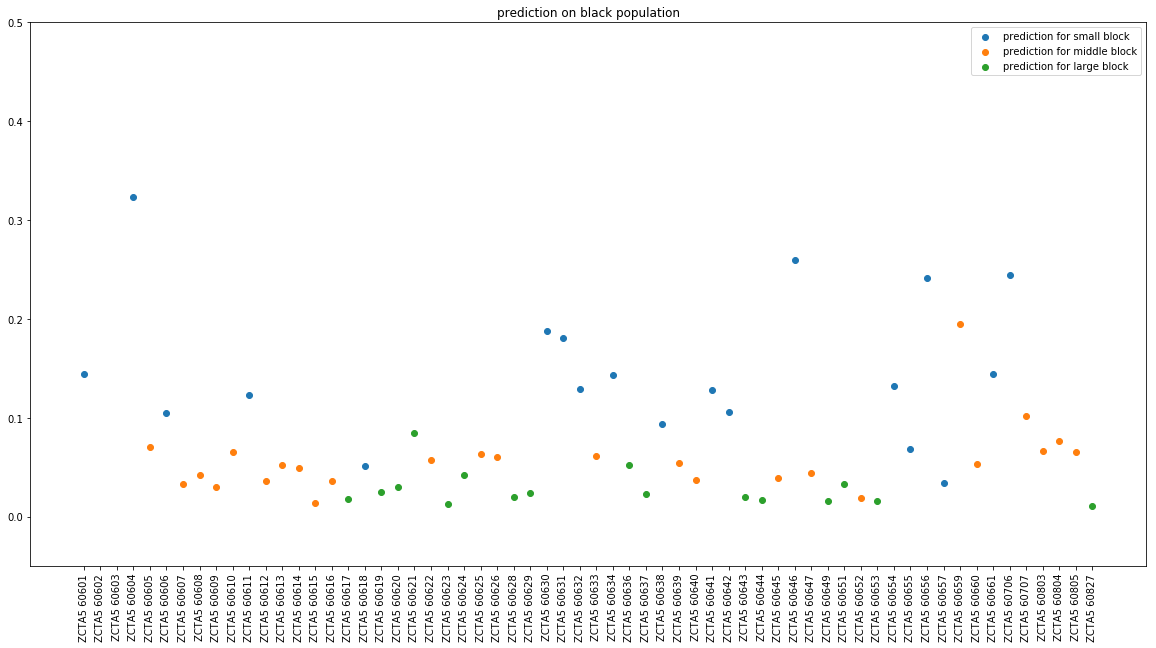
\includegraphics[width=1.2\textwidth]{graph3.png} 
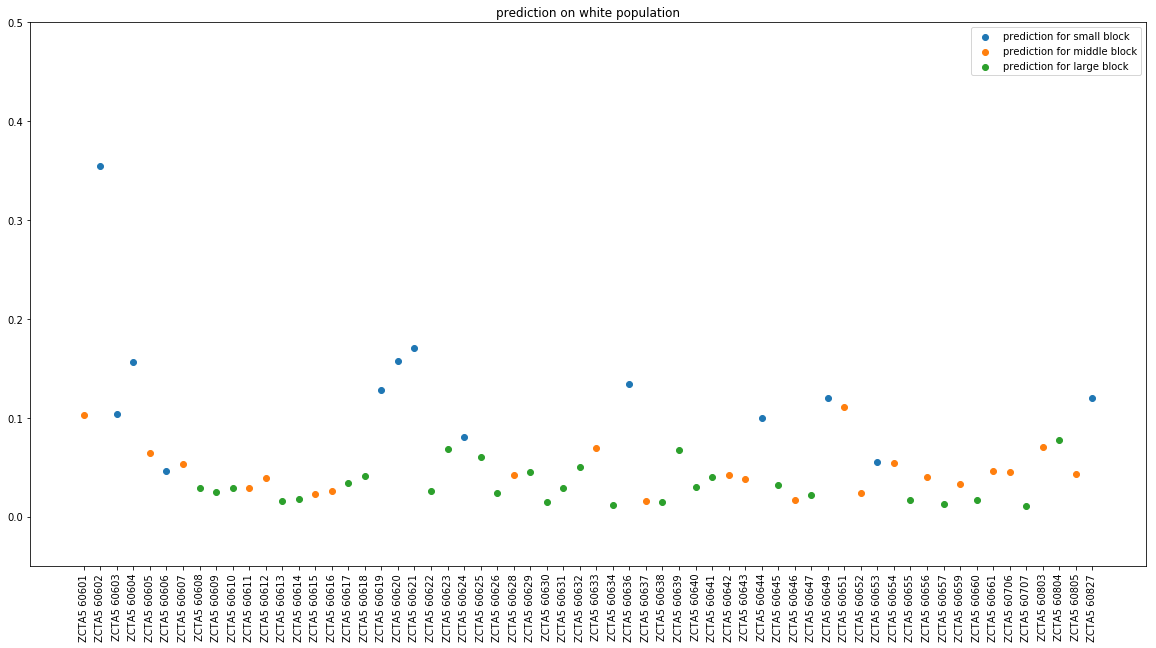
\includegraphics[width=1.2\textwidth]{graph4.png} 
\end{figure}
\clearpage
\centerline{{\color{white} 100} Table 3. Error rate for blacks and whites grouped by year}
\begin{table}[!h]
\begin{tabular}{lrrrrrr}
\toprule
{} &      2012 &      2013 &      2014 &      2015 &      2016 &      2017 \\
error rate for blacks &           &           &           &           &           &           \\
\midrule
small block           &  0.125388 &  0.161906 &  0.359161 &  0.145573 &  0.184917 &  0.198986 \\
medium block          &  0.056114 &  0.057022 &  0.071867 &  0.053815 &  0.072219 &  0.055366 \\
large block           &  0.028683 &  0.027910 &  0.022013 &  0.036036 &  0.024018 &  0.025191 \\
weighted average      &  0.034291 &  0.032680 &  0.030119 &  0.039930 &  0.030736 &  0.028752 \\
\bottomrule
\end{tabular}

\begin{tabular}{lrrrrrr}
\toprule
{} &      2012 &      2013 &      2014 &      2015 &      2016 &      2017 \\
error rate for whites &           &           &           &           &           &           \\
\midrule
small block           &  0.116622 &  0.150013 &  0.085454 &  0.168157 &  0.169404 &  0.107041 \\
medium block          &  0.048756 &  0.046920 &  0.044531 &  0.051271 &  0.049408 &  0.037956 \\
large block           &  0.055365 &  0.031297 &  0.032803 &  0.024092 &  0.020783 &  0.026411 \\
weighted average      &  0.053757 &  0.036604 &  0.032497 &  0.030143 &  0.027401 &  0.028901 \\
\bottomrule
\end{tabular}
\end{table}

\subsection{Discussion on Income}
\ \ \ \ This section focus on the impact of income factor on people's migration decision and its significance to the model.
\subsubsection{The choice of income}
\ \ \ \ In the previous part, we use mean income to represent the $income$ variable in the model. However, according to the statistics of income data (see Appendix Table 2), the values of 25, 50, 75 percentile and the mean of median income for 62 blocks in Chicago are significantly lower than those of mean income, suggesting that there may exist non-negligible income inequality. If that's the case, mean income may not be a good representation for the income variable when people consider migration. Table 4 compares the prediction error rate using different definition of income.
\par {\color{white} 100}
\par \centerline{{\color{white} 100} Table 4. Weighted average error rate using different definition of income}
\begin{table}[!h]
\begin{tabular}{lrrrrrr}
\toprule
{} &      2012 &      2013 &      2014 &      2015 &      2016 &      2017 \\
error rate for blacks &           &           &           &           &           &           \\
\midrule
mean income      &  0.034291 &  0.032680 &  0.030119 &  0.039930 &  0.030736 &  0.028752 \\
median income      &  0.029682 &  0.029998 &  0.027340 &  0.037251 &  0.028384 &  0.026461 \\
\bottomrule
\end{tabular}
\begin{tabular}{lrrrrrr}
\toprule
{} &      2012 &      2013 &      2014 &      2015 &      2016 &      2017 \\
error rate for whites &           &           &           &           &           &           \\
\midrule
mean income      &  0.053757 &  0.036604 &  0.032497 &  0.030143 &  0.027401 &  0.028901 \\
median income      &  0.053647 &  0.035663 &  0.031120 &  0.030095 &  0.026871 &  0.029055 \\
\bottomrule
\end{tabular}
\end{table}
\par As is shown in the table, the weighted average error rate for prediction on black population is reduced by about 0.3\% using median income, which is a 10\% reduction to previous results. Meanwhile, the weighted average error rates for prediction on white population are similar using different definitions. A possible reason is that the general income level of blacks is relatively lower and thus they pay more attention to the structure of income in the block. If that's the case, the model matches people's way of thinking better by switching to median income. On the other hand, whites may be more concerned about general income level of the block. As a result, mean income and median income have similar explanatory power.
\subsubsection{The significance of income}
\ \ \ \ Although using median income can improve the performance of the model, the significance of including income in the model hasn't been shown. This part will test the improvement caused by including income in the model. I train the model again while fixing $\beta_1$ at zero, and compare the prediction with previous one using median income. Table 5 summarizes the weighted average error rate of those two predictions.
\par {\color{white} 100}
\par \centerline{{\color{white} 100} Table 5. Weighted average error rate excluding and including income}
\begin{table}[!h]
\begin{tabular}{lrrrrrr}
\toprule
{} &      2012 &      2013 &      2014 &      2015 &      2016 &      2017 \\
error rate for blacks &           &           &           &           &           &           \\
\midrule
without income      &  0.032677 &  0.031590 &  0.030051 &  0.039740 &  0.028725 &  0.027953 \\
median income      &  0.029682 &  0.029998 &  0.027340 &  0.037251 &  0.028384 &  0.026461 \\
\bottomrule
\end{tabular}
\begin{tabular}{lrrrrrr}
\toprule
{} &      2012 &      2013 &      2014 &      2015 &      2016 &      2017 \\
error rate for whites &           &           &           &           &           &           \\
\midrule
without income      &  0.032677 &  0.031590 &  0.030051 &  0.039740 &  0.028725 &  0.027953 \\
median income      &  0.053647 &  0.035663 &  0.031120 &  0.030095 &  0.026871 &  0.029055 \\
\bottomrule
\end{tabular}
\end{table}
\par As is shown in the table, including median income improves the performance of prediction on black population but makes similar or even worse prediction on white population. The reason we mentioned last part might also explain the phenomenon here. Since the income of whites is high, the marginal utility of wealth is low and has little impact on their decision to move. The major factor affecting their migration decision is the environment of new neighborhood, which is percentage of whites in our model. 
\subsection{Discussion on homophily}
\ \ \ \ In section 2.1, I use exact percentage of specific ethnic group to represent the $homophily$ variable in the model. In this part, I will use a dummy variable to represent homophily variable. That is:
\begin{equation}
homophily=\left\{
\begin{aligned}
1 & \ if\ percentage > \phi & \\
& & \\
0 & \ otherwise & \\
\end{aligned}
\right.
\end{equation}
\par $\phi$ is a new parameter needs to be found by training. Table 6 compares the prediction error rate using exact percentage and dummy variable.
\par {\color{white} 100}
\par \centerline{{\color{white} 100} Table 6. Weighted average error rate using different definition of homophily}
\begin{table}[!h]
\begin{tabular}{lrrrrrr}
\toprule
{} &      2012 &      2013 &      2014 &      2015 &      2016 &      2017 \\
error rate for blacks &           &           &           &           &           &           \\
\midrule
dummy variable      &  0.031155 &  0.030966 &  0.027868 &  0.038100 &  0.030891 &  0.030227 \\
percentage      &  0.029682 &  0.029998 &  0.027340 &  0.037251 &  0.028384 &  0.026461 \\
\bottomrule
\end{tabular}
\begin{tabular}{lrrrrrr}
\toprule
{} &      2012 &      2013 &      2014 &      2015 &      2016 &      2017 \\
error rate for whites &           &           &           &           &           &           \\
\midrule
dummy variable      &  0.053519 &  0.035693 &  0.033935 &  0.030332 &  0.026238 &  0.030386 \\
percentage      &  0.053647 &  0.035663 &  0.031120 &  0.030095 &  0.026871 &  0.029055 \\
\bottomrule
\end{tabular}
\end{table}
\par As is shown in the table, the weighted average error rates for prediction on both blacks and whites are similar using different definitions. This finding suggests people might be not so sensitive to the population composition. They may only care about the general population composition of the block. It is reasonable because people have limited access to accurate statistics of population composition of every block.

\section{Appendix}
\begin{tabular}{llrrrr}
\toprule
           & Year &         2011 &         2012 &         2013 &         2014 \\
\midrule
 black population & count &      62 &      62 &      62 &      62 \\           & mean &   15064.016129 &   14865.258065 &   14617.032258 &   14478.758065 \\           & std &   19163.612657 &   18702.157889 &   18425.133138 &   18180.946499 \\           & min &       0 &       0 &       0 &      10 \\           & 25\% &    1827.75 &    1859.75 &    1700.75 &    1669.5 \\           & 50\% &    4427.5 &    4494 &    4347.5 &    4233 \\           & 75\% &   25403.5 &   25655.25 &   25904.25 &   25079.25 \\           & max &   75869 &   72649 &   71002 &   69652 \\black rate & count &      62 &      62 &      62 &      62 \\           & mean &       0.300237 &       0.299945 &       0.295957 &       0.293773 \\           & std &       0.342763 &       0.344000 &       0.342762 &       0.341311 \\           & min &       0 &       0 &       0 &       0.004815 \\           & 25\% &       0.040515 &       0.038981 &       0.037856 &       0.039869 \\           & 50\% &       0.165595 &       0.164146 &       0.156558 &       0.153084 \\           & 75\% &       0.533097 &       0.536640 &       0.535809 &       0.526432 \\           & max &       0.979562 &       0.978504 &       0.974338 &       0.971858 \\white population & count &      62 &      62 &      62 &      62 \\           & mean &   21267.048387 &   22291.967742 &   22753.032258 &   23071.645161 \\           & std &   17689.779441 &   18676.730468 &   19134.622313 &   19356.340396 \\           & min &     321 &     351 &     339 &     326 \\           & 25\% &    6317 &    6894.5 &    6852.75 &    7276 \\           & 50\% &   19992.5 &   21155.5 &   21010.5 &   20897 \\           & 75\% &   32268.25 &   34559.25 &   35065.5 &   36921.25 \\           & max &   63391 &   70518 &   75860 &   76907 \\white rate & count &      62 &      62 &      62 &      62 \\           & mean &       0.507465 &       0.518405 &       0.523778 &       0.526007 \\           & std &       0.291174 &       0.291052 &       0.293417 &       0.292847 \\           & min &       0.006839 &       0.007517 &       0.008857 &       0.008296 \\           & 25\% &       0.274583 &       0.290387 &       0.287005 &       0.287622 \\           & 50\% &       0.583600 &       0.591050 &       0.609351 &       0.614811 \\           & 75\% &       0.738630 &       0.749449 &       0.756871 &       0.758110 \\           & max &       0.905394 &       0.922888 &       0.923553 &       0.931595 \\total population & count &      62 &      62 &      62 &      62 \\           & mean &   46861.516129 &   46900.354839 &   46969.967742 &   47084.951613 \\           & std &   27147.057295 &   26847.490848 &   26712.831372 &   26696.120889 \\           & min &     393 &     428 &     415 &     419 \\           & 25\% &   27865.25 &   27853.5 &   28208.25 &   28108.25 \\           & 50\% &   43883.5 &   43566 &   44078 &   44079.5 \\           & 75\% &   67363.75 &   66965.75 &   67296.5 &   67579.5 \\           & max &  112376 &  111893 &  113833 &  115013 \\
\bottomrule
\end{tabular}
\begin{tabular}{llrrrr}
\toprule          & Year &         2015 &         2016 &         2017 & \\
\midrule

black population & count &      62 &      62 &      62 \\           & mean &   14262.048387 &   14113.467742 &   13965.903226 \\           & std &   17814.784187 &   17585.214503 &   17390.753978 \\           & min &      12 &      28 &      11 \\           & 25\% &    1642 &    1740 &    1702.75 \\           & 50\% &    4372.5 &    4540.5 &    4435 \\           & 75\% &   24041.25 &   23277.5 &   22807.5 \\           & max &   67353 &   66942 &   66537 \\black rate & count &      62 &      62 &      62 \\           & mean &       0.292148 &       0.291418 &       0.289013 \\           & std &       0.340509 &       0.338358 &       0.336210 \\           & min &       0.006652 &       0.005296 &       0.006414 \\           & 25\% &       0.036672 &       0.040344 &       0.037911 \\           & 50\% &       0.145420 &       0.139971 &       0.131808 \\           & 75\% &       0.540221 &       0.542120 &       0.515845 \\           & max &       0.969154 &       0.967368 &       0.963408 \\white population & count &      62 &      62 &      62 \\           & mean &   23253.419355 &   23186.838710 &   23405.629032 \\           & std &   19442.414740 &   19317.192039 &   19378.972083 \\           & min &     380 &     381 &     418 \\           & 25\% &    7770.5 &    7838.5 &    7998.25 \\           & 50\% &   21440 &   21431.5 &   21683.5 \\           & 75\% &   37566.25 &   37377 &   35479.75 \\           & max &   78374 &   77910 &   76981 \\white rate & count &      62 &      62 &      62 \\           & mean &       0.525297 &       0.520550 &       0.522409 \\           & std &       0.291600 &       0.288395 &       0.287907 \\           & min &       0.012033 &       0.013292 &       0.015161 \\           & 25\% &       0.275991 &       0.278185 &       0.282083 \\           & 50\% &       0.622566 &       0.613404 &       0.603769 \\           & 75\% &       0.747336 &       0.741069 &       0.753429 \\           & max &       0.924655 &       0.913662 &       0.903827 \\total population & count &      62 &      62 &      62 & \\           & mean &   47171.822581 &   47098.580645 &   47222.306452 & \\           & std &   26688.734509 &   26491.581774 &   26485.770365 & \\           & min &     545 &     619 &     668 & \\           & 25\% &   28311 &   28272.75 &   28874 & \\           & 50\% &   44155 &   44334.5 &   43902.5 & \\           & 75\% &   67448 &   67829.75 &   68179 & \\           & max &  114982 &  115104 &  114129 & \\
\bottomrule
\end{tabular}
\par
\centerline{{\color{white} 100} Table 1. Statistics of population data (grouped by year)}
\par
\begin{tabular}{llrrrr}
\toprule      & Year &         2011 &         2012 &         2013 &         2014 \\
\midrule
mean income & count &      62 &      62 &      62 &      62 \\              & mean &   75693.758065 &   75549.274194 &   77636.403226 &   77727.790323 \\              & std &   34019.002717 &   33151.315275 &   38144.700123 &   38884.730418 \\              & min &   33534 &   33049 &   31965 &   31288 \\              & 25\% &   50327.5 &   49622.25 &   48580 &   49505.25 \\              & 50\% &   67383.5 &   67002 &   65965 &   67309 \\              & 75\% &   91505.25 &   94433.25 &   97909 &   97961.75 \\              & max &  169005 &  166752 &  214918 &  232790 \\median income & count &      62 &      62 &      62 &      62 \\              & mean &   55054.096774 &   54807.516129 &   55478.274194 &   56351.161290 \\              & std &   22353.940314 &   22353.640437 &   24266.105957 &   26054.531192 \\              & min &   19692 &   19623 &   19548 &   19190 \\              & 25\% &   38611.25 &   38117.75 &   37740.25 &   37055.75 \\              & 50\% &   50999 &   50499.5 &   50383.5 &   51486.5 \\              & 75\% &   69348.25 &   70755 &   71707.75 &   71819.25 \\              & max &  109375 &  107056 &  132188 &  155750 \\
\bottomrule
\end{tabular}

\begin{tabular}{llrrrr}
\toprule              & Year &         2015 &         2016 &         2017 & \\
\midrule

mean\_income & count &      62 &      62 &      62 & \\              & mean &   79947.290323 &   82670.741935 &   88015.967742 & \\              & std &   43090.234148 &   41553.540018 &   45318.732623 & \\              & min &   30458 &   31845 &   32722 \\              & 25\% &   50204.75 &   52622.25 &   54778.25 & \\              & 50\% &   68753.5 &   72261 &   74314 & \\              & 75\% &  100561.5 &  104907.75 &  114223.5 & \\              & max &  261215 &  224642 &  221184 & \\median\_income & count &      62 &      62 &      62 & \\              & mean &   56931.064516 &   59591.951613 &   62405.145161 & \\              & std &   26768.025370 &   28867.416900 &   29962.273691 & \\              & min &   19832 &   20150 &   19845 & \\              & 25\% &   36291.25 &   37166.25 &   38857.75 & \\              & 50\% &   52264.5 &   53835.5 &   56027 & \\              & 75\% &   74683.75 &   79083.5 &   85457 & \\              & max &  151731 &  150125 &  140114 & \\
\bottomrule
\end{tabular}
\centerline{{\color{white} 100} Table 2. Statistics of income data (grouped by year)}


\bibliographystyle{plain}
\bibliography{references}
\end{document}
